\documentclass[margin=0px]{article}

\usepackage{listings}
\usepackage[utf8]{inputenc}
\usepackage{graphicx}
\usepackage{float}
\usepackage[a4paper, margin=0.7in]{geometry}
\usepackage{subcaption}
\usepackage{amsthm}
\usepackage{amssymb}
\usepackage{amsmath}
\usepackage{fancyhdr}
\usepackage{setspace}

\onehalfspacing

\renewcommand{\figurename}{ábra}
\newenvironment{tetel}[1]{\paragraph{#1 \\}}{}
\newcommand{\R}{\mathbb{R}}

\pagestyle{fancy}
\lhead{\it{PTI BSc Záróvizsga tételek}}
\rhead{2. Differenciál- és integrálszámítás}

\title{\textbf{{\Large ELTE IK - Programtervező Informatikus BSc} \vspace{0.2cm} \\ {\huge Záróvizsga tételek}} \vspace{0.3cm} \\ 2. Differenciál- és integrálszámítás}
\author{}
\date{}

\begin{document}
\maketitle

\begin{tetel}{Differenciál- és integrálszámítás}
    Függvények deriválhatósága. Parciális derivált, totális derivált. Gradiens, Jacobi-mátrix. Függvényvizsgálat, szélsőérték. Riemann-integrál, parciális integrálás, integrálás helyettesítéssel. Newton-Leibniz-formula.
\end{tetel}

\section{Függvények deriválhatósága}
\begin{description}
    \item[Differenciálhatóság] \hfill \\
        $ 1 \leq n, m \in \mathbb{N}, \quad 1 \leq p,q \leq +\infty,$

        $ (\R^n, \lVert . \rVert_p)$ és $ (\R^m, \lVert . \rVert_q)$ normált terek

        $ f \in \R^n \rightarrow \R^m, \ a \in intD_f $

        Az $f$ függvény differenciálható az $a$ pontban ($ f \in D\{a\}$) , ha\\
        létezik olyan $ L \in L(\R^n, \R^m)$ korlátos lineáris leképezés és olyan $ \eta \in \R^n \rightarrow \R^m $ függvény, hogy :
        \begin{align*}
            f(a+h)-f(a) = L(h)+\eta(h)\cdot \lVert h\rVert_p \quad ( h \in \R^n, a+h \in D_f)
        \end{align*}
        ahol
        \begin{align*}
            \eta(h) \longrightarrow 0 \quad (\lVert h\rVert_p \rightarrow 0)
        \end{align*}

        Más szóval:

        \[ \dfrac{f(a+h)-f(a)-L(h)}{\lVert h\rVert_p} \longrightarrow 0 \quad (\lVert h\rVert_p \rightarrow 0)\]
        \\\\
        Amennyiben $\forall a\in intD_f : f \in D\{a\} $, akkor az $f$ differenciálható ($f \in D$)
        \\\\
        \textit{
            Megjegyzés:\\
            A $ \mathbb{K}$ test feletti $ (X, \lVert.\rVert_\bigstar )$,  $ (X, \lVert.\rVert_\heartsuit )$ normált terek közötti folytonos leképezés, korlátos lineáris leképezés, ha
            \begin{itemize}
                \item lineáris, azaz
                      \begin{align*}
                          f(x+\lambda y) = f(x) + \lambda f(y) \quad (x,y \in X, \lambda \in \mathbb{K})
                      \end{align*}
                \item korlátos, azaz
                      \begin{align*}
                          \exists M \geq 0 : \lVert f(x) \rVert_\heartsuit \leq M\lVert x \rVert_\bigstar \quad (x \in X)
                      \end{align*}
            \end{itemize}
        }
    \item[Derivált] \hfill \\
        $f\in\R^n\rightarrow\R^m $ függvény differenciálható egy $a\in intD_f$ pontban \\
        $ \Rightarrow \exists! L\in L(\R^n,\R^m)$ korlátos lineáris leképezés

        Ezt az egyértelműen létező $L \in L(\R^n,\R^m) $ korlátos lineáris leképezést az $f$ függvény $a$ pontbeli deriváltjának nevezzük, és $f'(a)$ szimbólummal jelöljük.
\end{description}

\section{Parciális derivált, Totális derivált}
\subsection{Parciális derivált}
\begin{description}
    \item[Definíció] \hfill \\
        Tekintsük a $ h \in \R^n \rightarrow \R $ függvényt és az $a = (a_1, ... , a_n) \in D_h $ vektort. Legyen
        \begin{align*}
            D_{h,i}^{(a)} := \{t \in \R : (a_1, ..., a_{i-1}, t, a_{i+1}, ..., a_n) \in D_h\} \quad (i = 1,...,n)
        \end{align*}
        És legyen:
        \begin{align*}
            h_{a,i} : D_{h,i}^{(a)} \rightarrow \R, \quad \textrm{ melyre: } \quad h_{a,i}(t) := h(a_1, ..., a_{i-1}, t, a_{i+1}, ..., a_n) \quad (t\in	D_{h,i}^{(a)} )
        \end{align*}
        A $h_{a,i}$ parciális függvények mind egyváltozós valós függvények ($h_{a,i} \in \R \rightarrow\R $)

        A $ h $ függvény az $a$-ban $i$-edig változó szerint parciálisan deriválható, ha $ h_{a,i} \in D\{a_i\} $. Ekkor:
        \begin{align*}
            \partial_ih(a) := h'_{a,i}(a_i)
        \end{align*}
        valós számot a $h$ függvény $a$-beli, $i$-edik változó szerinti parcális deriváltjának nevezzük.
    \item[Parciális derivált függvény] \hfill \\
        Tegyük fel, hogy az előző $h$ függvényre:
        \begin{align*}
            D_{h,i} := \{a \in D_h : \textrm{létezik a } \partial_ih(a) \textrm{parciáis derivált}\} \neq \emptyset \qquad (i=1,...,n)
        \end{align*}
        Ekkor a
        \begin{align*}
            x \mapsto \partial_ih(x) \quad (x\in D_{h,i})
        \end{align*}
        függvényt a $h$ függvény $i$-edik változó szerinti parciális deriváltfüggvényének nevezzük, és a $\partial_ih$ szimbólummal jelöljük.
    \item[Differenciálhatóság és parciális differenciálhatóság] \hfill
        \begin{itemize}
            \item Differenciálhatóság $\Rightarrow$ parciális differenciálhatóság \\
                  $ 1 \leq n \in \mathbb{N}, \ h \in \R^n \rightarrow \R, $ és $h\in D\{a\} \ (a \in D_h) $ \\
                  $\Rightarrow \forall i = 1,...,n$ : a $h$ függvény $i$-edik változó szerint parciálisan differenciálható az $a$ pontban, és
                  \begin{align*}
                      \textrm{grad}h(a) = (\partial_1h(a), ..., \partial_nh(a))
                  \end{align*}

            \item Differenciálhatóság $\Leftarrow$ parciális differenciálhatóság \\
                  $ 1 \leq n \in \mathbb{N}, \ h \in \R^n \rightarrow \R, $ és $ a \in intD_h $ \\
                  Valamilyen $i = 1,...,n$ esetén:
                  \begin{itemize}
                      \item Tetszőleges $ x \in K_r(a) $ ($r > 0$ alkalmas) helyen léteznek a $ \partial_jh(x)$ parciális deriváltak $ (i \neq j = 1,...,n)$ és ezek folytonosak
                      \item $\exists \ \partial_ih(a)$ parciális derivált
                  \end{itemize}
                  $\Rightarrow h\in D(a)$
        \end{itemize}
\end{description}
\subsection{Totális derivált}
\rm Az $ f: \R^p \to \R^q $ függvényt {\it (totálisan) differenciálhatónak\,} mondjuk az $a\in D(f)$ pontban,
ha létezik egy $ L: \R^p \to \R^q $ lineáris leképezés úgy, hogy
$$
    \lim_{x\to a}\frac{f(x)-f(a)-L(x-a)}{\|x-a\|}=0.
$$
Az $L$ lineáris leképezést az $f$ függvény $a$ pontbeli {\it differenciáljának,} az $L$ leképezés $M_L$ mátrixát pedig
$f$ $a$-beli {\it differenciálhányadosának vagy Jacobi-mátrixának\,} nevezzük. Jelölés: $L=Df(a)$, illetve $M_L=f'(a)$.

Valós $f$ esetén ($q=1$) az $f'(a)$ Jacobi-mátrix $1\times p$ típusú, azaz $p$ dimenziós sorvektor. Ebben az esetben az $a$
pontbeli Jacobi-mátrix helyett az $a$ pontbeli {\it gradiens {\rm vagy} gradiensvektor\,} elnevezés és az $f'(a)=\operatorname{grad} f(a)$
jelölés is használatos.

\section{Jacobi-mátrix, gradiens}
\begin{description}
    \item[Jacobi-mátrix] \hfill \\
        Az előzőekben szereplő $L := f'(a) $ korlátos lineáris leképezéshez $ \exists!A\in\R^{m\times n}$ mátrix, melyre:
        \begin{align*}
            L(x) = Ax \quad (x\in\R^n)
        \end{align*}
        Ezért:
        $ f'(a) := A $\\
        az $f$ függvény $a$-beli deriváltja vagy derivált mátrixa, más néven Jacobi-mátrixa.
    \item[Gradiens] \hfill \\
        $m = 1$ esetén : $ f \in \R^n \rightarrow \R $
        \begin{align*}
            \textrm{grad}f(a) := f'(a) \in \R^{1\times n} \approx \R^n
        \end{align*}
        Tehát ebben az esetben az $f'(a)$ Jacobi-mátrix tekinthető egy $\R^n$-beli vektornak, amit az $f$ függvény $a$-beli gradiensének nevezünk.
        \\\\
        Ha $ D := \{a \in D_f : f \in D\{a\} \} $, akkor az
        \begin{align*}
            x \mapsto \textrm{grad}f(x) \in \R^n \quad (x \in D)
        \end{align*}
        függvényt az $f$ függvény gradiensének nevezzük, és grad$f \in \R^n \rightarrow \R^n$ jelöljük.
    \item[Gradiens mint Jacobi-mátrix sora] \hfill \\
        Legyen $1 \leq n, m \in \mathbb{N}$. Az $f = (f_1, ..., f_m) \in \R^n \rightarrow \R^m$ függvény akkor és csak akkor differenciálható az $ a \in intD_f$ helyen, ha minden $ i = 1, ..., m $ esetén az
        $f_i \in \R^n \rightarrow \R$  koordináta-függvény differenciálható az $a$-ban.

        Ha $f \in D\{a\}$, akkor az $f'(a)$ Jacobi-mátrix a következő alakú:
        \begin{align*}
            f'(a) =
            \begin{bmatrix}
                \textrm{grad}f_{1}(a) \\
                \textrm{grad}f_{2}(a) \\
                \vdots                \\
                \textrm{grad}f_{m}(a) \\
            \end{bmatrix}
        \end{align*}
\end{description}

\section{Szélsőérték, függvényvizsgálat}
\subsection{Szélsőérték}
$ f \in \R \rightarrow \R, a \in D_f$
\begin{description}
    \item[Lokális maximum] \hfill \\
        $f$-nek $a$-ban lokális maximuma van, ha alkalmas $ r > 0$ mellett: \\
        $ f(x) \leq f(a) \qquad (x\in D_f, |x-a|<r)$
    \item[Lokális minimum] \hfill \\
        $f$-nek $a$-ban lokális minimuma van, ha alkalmas $ r > 0$ mellett: \\
        $ f(x) \geq f(a) \qquad (x\in D_f, |x-a|<r)$
    \item[Abszolút maximum] \hfill \\
        $f$-nek $a$-ban abszolút maximuma van, ha: \\
        $ f(x) \leq f(a) \qquad (x\in D_f)$
    \item[Abszolút mimimum] \hfill \\
        $f$-nek $a$-ban abszolút minumuma van, ha: \\
        $ f(x) \geq f(a) \qquad (x\in D_f)$
    \item[Lokális szélsőérték] \hfill \\
        $f$-nek $a$-ban lokális szélsőértéke van, ha $a$-ban lokális minimuma vagy maximuma van.
    \item[Abszolút szélsőérték] \hfill \\
        $f$-nek $a$-ban abszolút szélsőértéke van, ha $a$-ban abszolút minimuma vagy maximuma van.
    \item[Elsőrendű szükséges feltétel (lokális szélsőértékre)] \hfill \\
        $f \in \R \rightarrow \R$ függvénynek $ a \in intD_f $ helyen lokális szélsőértéke van, és $ f \in D\{a\}$ \\
        $ \Rightarrow f'\{a\} = 0 $
\end{description}
Az előbbi tétel segítségével már nem nehéz belátni a differenciálható függvények vizsgálata szempontjából alapvető fontosságú ún. középérték-tételeket

\begin{description}
    \item[Rolle-tétel] \hfill \\
        $ a,b \in \R \ (a<b), \ f:[a,b] \rightarrow \R, \ f\in C$, és \\
        $ \forall x\in (a,b) : f\in D\{x\} $ és $ f(a) = f(b) $ \\
        $ \Rightarrow \exists \ \xi \in (a,b) : f'(\xi) = 0 $
    \item[Lagrange-féle középértéktétel] \hfill \\
        $ a,b \in \R \ (a<b), \ f:[a,b] \rightarrow \R, \ f\in C$, és \\
        $ \forall x\in (a,b) : f\in D\{x\} $ \\
        $ \Rightarrow \exists \ \xi \in (a,b) : f'(\xi) = \dfrac{f(b)-f(a)}{b-a}  $
    \item[Cauchy-féle középértéktétel] \hfill \\
        $ a,b \in \R \ (a<b), \ f,g:[a,b] \rightarrow \R, \ f,g\in C$, és \\
        $ \forall x\in (a,b) : f,g\in D\{x\} $ \\
        $ \Rightarrow \exists \ \xi \in (a,b) :$ \\
        $ (f(b)-f(a))\cdot g'(\xi) = (g(b)-g(a)\cdot f'(\xi) $
\end{description}
\begin{description}
    \item[Jelváltás] \hfill \\
        $ f \in \R \rightarrow \R,\ a \in intD_f $ és $ f(a) = 0, \ ( K_r(a) \subset D_f, r > 0 ) $
        \begin{enumerate}
            \item $f$ függvénynek $ (-,+) $ jelváltása van, ha \\
                  $ f(x) \leq 0 \leq f(t), \quad (x,t \in K_r(a), \ x<a<t) $
            \item $f$ függvénynek $ (+,-) $ jelváltása van, ha \\
                  $ f(x) \geq 0 \geq f(t), \quad (x,t \in K_r(a), \ x<a<t) $
        \end{enumerate}
    \item[Elsőrendű elégséges feltétel] \hfill \\
        $ f \in \R \rightarrow \R, \ a \in intD_f $ és $ f\in D\{x\}, \ (x \in K_r(a) \subset D_f, r > 0 ) $
        \begin{enumerate}
            \item $f'$-nak az $a$-ban $(+,-)$ jelváltása van $\Rightarrow f$-nek $a$-ban lokális maximuma van.
            \item $f'$-nak az $a$-ban $(-,+)$ jelváltása van $\Rightarrow f$-nek $a$-ban lokális minimuma van.
        \end{enumerate}
\end{description}
\subsection{Monotonitás}
$ f\in \R \rightarrow \R $
\begin{description}
    \item[Monoton növekedés] \hfill \\
        $ f $ monoton növő ($\nearrow$), ha $\forall x,t \in D_f, \ x < t : f(x) \leq f(t) $. \\
        Amennyiben $  f(x) < f(t) $, akkor $f$ szigorúan monoton növő ($\uparrow$).
    \item[Monoton fogyás (csökkenés)] \hfill \\
        $ f $ monoton fogyó ($\searrow$), ha $\forall x,t \in D_f, \ x < t : f(x) \geq f(t) $. \\
        Amennyiben $  f(x) > f(t) $, akkor $f$ szigorúan monoton fogyó ($\downarrow$).
    \item[Derivált és monotonitás kapcsolata] \hfill \\
        $ I \subset \R $ nyílt intervallum, $ f:I\rightarrow \R, \ f \in D$\\
        $\Rightarrow$
        \begin{enumerate}
            \item $ f \nearrow \ \Leftrightarrow \ f' \geq 0$
            \item $ f \searrow \ \Leftrightarrow \ f' \leq 0$
            \item $ f \ konstans \ \Leftrightarrow \ \forall x \in I : f'(x) = 0$
            \item $ \forall x \in I : f'(x) > 0 \ \Rightarrow  \ f \uparrow $
            \item $ \forall x \in I : f'(x) < 0 \ \Rightarrow  \ f \downarrow $
        \end{enumerate}
\end{description}
\subsection{Alaki viszonyok}
\begin{description}
    \item[Konvexitás, konkávitás] \hfill \\
        $ I \subset \R $ intervallum, $ f:I\rightarrow \R $
        \begin{itemize}
            \item $f$ konvex, ha \\
                  $\forall a,b \in I \quad \forall 0\leq \lambda \leq 1: f(\lambda a+(1-\lambda)b) \leq  \lambda f(a) + (1-\lambda)f(b)$
            \item $f$ konkáv, ha \\
                  $\forall a,b \in I \quad \forall 0\leq \lambda \leq 1: f(\lambda a+(1-\lambda)b) \geq  \lambda f(a) + (1-\lambda)f(b)$
        \end{itemize}
        \begin{figure}[H]
            \centering
            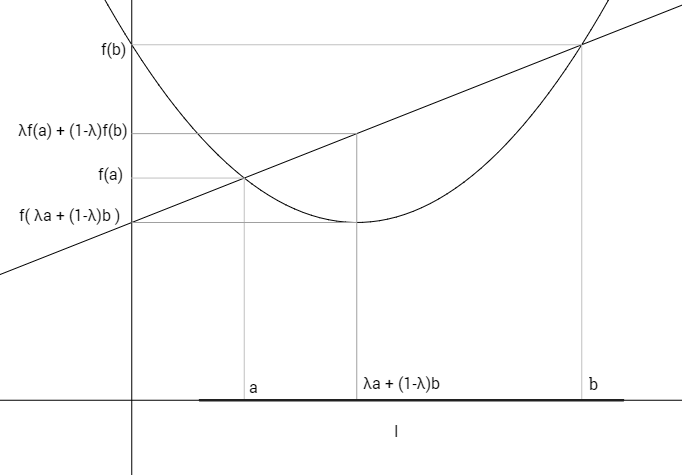
\includegraphics[width=0.6\textwidth]{img/konvex.png}
            \caption{Konvex függvény}
        \end{figure}
    \item[Konvexitás és derivált] \hfill \\
        $ I \subset \R $ nyílt intervallum, $f:I\rightarrow \R, \ f \in D $
        \begin{itemize}
            \item $f$ konvex $ \Leftrightarrow f' \nearrow $
            \item $f$ konkáv $ \Leftrightarrow f' \searrow $
        \end{itemize}
    \item[Inflexió] \hfill \\
        $ f \in \R \rightarrow \R, \ a \in intD_f, \ f \in D\{a\} $:
        \begin{description}
            \item[Pontbeli érintő] \hfill \\
                $ e_a(x) := f(a) + f'(a)(x-a) \quad (x\in\R)$
            \item[Inflexió] \hfill \\
                $ f$-nek az $a$-ban inflexiója van, ha az $f - e_a(f) $ az $a$-ban jelet vált.
        \end{description}
        \begin{figure}[H]
            \begin{subfigure}{.33\textwidth}
                \centering
                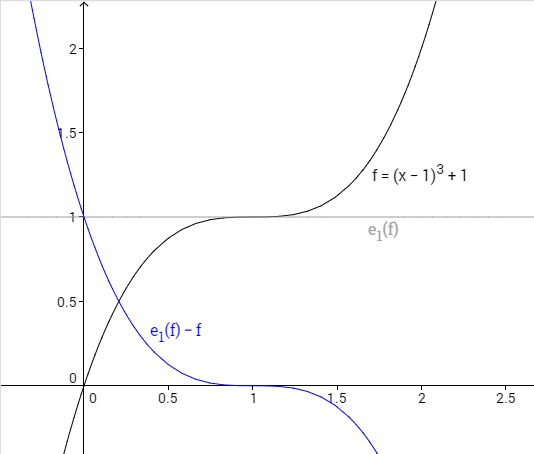
\includegraphics[width=0.7\textwidth]{img/inflexio_x3.png}
                \caption{$x^3$ függvény inflexiója}
            \end{subfigure}
            \begin{subfigure}{.33\textwidth}
                \centering
                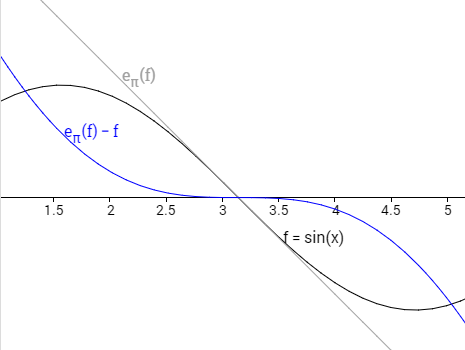
\includegraphics[width=0.7\textwidth]{img/inflexio_sin.png}
                \caption{szinusz függvény inflexiója}
            \end{subfigure}
            \begin{subfigure}{.33\textwidth}
                \centering
                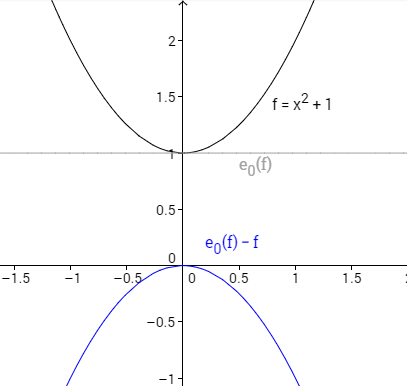
\includegraphics[width=0.7\textwidth]{img/inflexio_x2.png}
                \caption{$x^2$-nek nincs inflexiója}
            \end{subfigure}
        \end{figure}
\end{description}
\subsection{Többször differenciálható függvények}
\begin{description}
    \item[Második derivált] \hfill \\
        $ f \in \R \rightarrow \R, \ a \in intD_f, $ és \\
        $ f \in D\{x\} \quad (x \in K_r(a), r>0)$, illetve $f' \in D\{a\}$ \\
        Ekkor $f$ az $a$-ban kétszer deriválható és $f''(a) := (f')'(a) $ az $f$ második deriváltja.
    \item[Differenciálás magasabb rendben] \hfill \\
        Hasonlóképpen az előzőhöz:\\
        $ f \in \R \rightarrow \R, \ a \in intD_f, $ és \\
        $ f \in D^n\{x\} \quad (x \in K_r(a), r>0)$, illetve $f^{(n)} \in D\{a\}, \ (1 \leq n \in \mathbb{N})$ \\
        Ekkor $f$ az $a$-ban $(n+1)$-szer deriválható és $f^{(n+1)}(a) := (f^{(n)})'(a) $ az $f \ (n+1)$-edik deriváltja.
    \item[Másodrendű elégséges feltétel (lokális szélsőérték létezésére)] \hfill \\
        $ f \in D^2\{a\}$ függvényre $f'(a) = 0$ és $f''(a) \neq 0 $ \\
        $ \Rightarrow f$-nek az $a$-ban szigorú lokális szélsőértéke van. \\
        Ha $f''(a) < 0 \Rightarrow $ szigorú lokális maximum. \\
        Ha $f''(a) > 0 \Rightarrow $ szigorú lokális minimum.
\end{description}
\section{Riemann-integrál, parciális integrálás, integrálás helyettesítéssel.}
\begin{description}
    \item[Primitív függvény] \hfill \\
        $ I \subset \R $ nyílt intervallum, $ f \in I \rightarrow \R $ \\
        Ha $ \exists  F:I\rightarrow\R $, hogy  $ F \in D $, $F' = f$ \\
        akkor $ F $ az $ f $ primitív függvénye.

    \item[Határozatlan integrál] \hfill \\
        Legyen $ \int{f} := \int f(x)dx :=  \{F:I \rightarrow \R, F \in D $
        és $ F' = f  \} $ az f határozatlan integrálja.

    \item[Határozott integrál (Riemann-integrál)] \hfill \\
        $ -\infty < a < b < \infty$
        $, f:[a,b] \rightarrow \R, f $ korlátos
        \begin{itemize}
            \item
                  A $ \tau \subset [a,b] $ felosztása, ha $ \tau $ véges és $ a,b \in \tau $ \\
                  Ekkor $ \tau = \{x_0, x_1, ..., x_n \} (n \in \mathbb{N}) $, ahol
                  $ a := x_0 < x_1 < ... < x_n := b$
            \item
                  $ m_i := m_i(f) := inf\{f(x): x_i \leq x \leq x_{i+1} \} (i = 0..n-1)$, illetve \\
                  $ M_i := M_i(f) := sup\{f(x): x_i \leq x \leq x_{i+1} \} (i = 0..n-1)$

                  és:

                  $ s(f, \tau) := \sum\limits_{i=0}^{n-1} m_i(x_{i+1} - x_i) $ - alsó összeg \\
                  $ S(f, \tau) := \sum\limits_{i=0}^{n-1} M_i(x_{i+1} - x_i) $ - felső összeg

            \item
                  $ \mathfrak{F} := \{ \tau \subset [a,b] $ felosztás $\}$
            \item
                  Az $ \{ s(f, \tau): \tau \in \mathfrak{F} \} $ felülről korlátos és $ \forall \mu \in \mathfrak{F} : S(f, \mu) $ felső korlát, illetve \\
                  Az $ \{ S(f, \tau): \tau \in \mathfrak{F} \} $ alulról korlátos és $ \forall \mu \in \mathfrak{F} : s(f, \mu) $ alsó korlát
            \item
                  Tehát legyen: \\ $ I_*(f) := sup\{ s(f,\tau) : \tau \in \mathfrak{F} \}$ - Darboux alsó index, és \\
                  $ I^*(f) := inf\{ S(f,\tau) : \tau \in \mathfrak{F} \}$ - Darboux felső index
        \end{itemize}

        $ \Rightarrow \forall \tau,\mu \in \mathfrak{F} : s(f, \tau) \leq I_*(f) \leq I^*(f) \leq S(f,\mu) $

        Az $ f $ függvény Riemann-integrálható ($ f \in R[a,b] $), ha $ I_*(f) = I^*(f) $, ekkor legyen \\
        $ \int_{a}^{b}f := \int_{[a,b]}f := \int_{a}^{b}f(x) dx := I_*(f) = I^*(f) $ az $f$ függvény Riemann-integrálja (határozott integrálja).

    \item[Parciális integrálás] \hfill
        \begin{itemize}
            \item Határozatlan esetben \hfill \\
                  $ I \subset \R $ nyílt intervallum, $ f,g : I \rightarrow \R $, $f,g \in D$ és \\
                  $ fg'$-nek van primitív függvénye (azaz $ \int fg' \neq \emptyset $)\\
                  $ \Rightarrow \int f'g \neq \emptyset $ és $ \int f'g = fg - \int fg' $
            \item Határozott esetben \hfill \\
                  $ f,g \in D[a,b] \\ f'g, f g' \in R[a,b] $ \\
                  $ \Rightarrow \int_a^b f'g = f(b)g(b) - f(a)g(a) - \int_a^b fg'$
        \end{itemize}

    \item[Integrálás helyettesítéssel] \hfill
        \begin{itemize}
            \item Határozatlan esetben \hfill \\
                  $ I,J \subset \R $ nyílt intervallumok, $g: I \rightarrow J,  g \in D, f:J \rightarrow \R, \int f \neq \emptyset $ \\
                  $\Rightarrow \int f \circ g\cdot g' \neq \emptyset $ és $ (\int f) \circ g = \int(f\circ g\cdot g') $
            \item Határozott esetben \hfill \\
                  $ f \in C[a,b], g : [\alpha,\beta] \rightarrow [a,b], g \in C^1[\alpha,\beta],$\\
                  $g(\alpha) = a, g(\beta) = b $ \\
                  $ \Rightarrow \int_a^b f = \int_{\alpha}^{\beta} (f\circ g \cdot g')$
        \end{itemize}
\end{description}
\section{Newton-Leibniz-formula}

$ f \in R[a,b], \exists F:[a,b] \rightarrow \R, F $ folytonos és $ F \in D\{x\}, F'(x) = f(x), (a < x < b) $ \\
$ \Rightarrow \int_a^b f = F(b) - F(a) $

\end{document}